\documentclass[a4paper,13pt]{extarticle}

% Khai báo các gói lệnh cần thiết
\usepackage{booktabs}
\usepackage{multirow}
\usepackage[utf8]{inputenc}
\usepackage[T5]{fontenc} % Font tiếng Việt
\usepackage[vietnamese]{babel} % Hỗ trợ quy tắc tiếng Việt
\usepackage{mathptmx} % Font Times New Roman giả lập
\usepackage{geometry} % Căn lề
\usepackage{graphicx} % Chèn ảnh (logo)
\usepackage{subcaption} % Hỗ trợ subfigure
\usepackage{tikz} % Vẽ khung bìa
\usepackage{listings}
\usetikzlibrary{calc}
\usepackage{pgfplots} % Vẽ sơ đồ so sánh
\pgfplotsset{compat=1.18}
\usepackage{anyfontsize} % Thay đổi cỡ chữ linh hoạt
\usepackage{setspace} % Giãn dòng
\usepackage{hyperref} % Hỗ trợ chèn link web
\usepackage{indentfirst} % Ép thụt đầu dòng cho đoạn văn đầu tiên sau tiêu đề
\usepackage{tabularx}
\usepackage{array}
\usepackage{url}
\usepackage{hyperref}
\usepackage{enumitem}
\usepackage{amsmath}
\usepackage{float}       % Bắt buộc phải có để dùng [H]
\usepackage{algorithm}   % Tạo khung thuật toán
\usepackage{algpseudocode}
\floatname{algorithm}{Giải thuật}
\renewcommand{\algorithmicrequire}{\textbf{Đầu vào:}}
\renewcommand{\algorithmicensure}{\textbf{Đầu ra:}}
\usepackage{xurl}


% Cấu hình lề trang (Chuẩn A4)
\geometry{
  top=2cm,
  bottom=2cm,
  left=3cm,
  right=2cm
}
% Lệnh vẽ khung viền (2 nét: nét đậm ngoài, nét mảnh trong)
\newcommand{\drawCoverFrame}{
    \begin{tikzpicture}[remember picture, overlay]
        % Nét đậm bên ngoài
        \draw[line width=2pt] 
            ($(current page.north west) + (2.5cm,-2.0cm)$) 
            rectangle 
            ($(current page.south east) + (-1.5cm,2.0cm)$);
        % Nét mảnh bên trong
        \draw[line width=0.5pt] 
            ($(current page.north west) + (2.6cm,-2.1cm)$) 
            rectangle 
            ($(current page.south east) + (-1.6cm,2.1cm)$);
    \end{tikzpicture}
}

% Cấu hình hiển thị code Python
\definecolor{codegreen}{rgb}{0,0.6,0}
\definecolor{codegray}{rgb}{0.5,0.5,0.5}
\definecolor{codepurple}{rgb}{0.58,0,0.82}
\definecolor{backcolour}{rgb}{0.97,0.97,0.97}
\lstdefinestyle{pythonstyle}{
    backgroundcolor=\color{backcolour},   
    commentstyle=\color{codegreen},
    keywordstyle=\color{blue}\bfseries,
    %numberstyle=\tiny\color{codegray},
    stringstyle=\color{codepurple},
    basicstyle=\ttfamily\footnotesize,
    breakatwhitespace=false,         
    breaklines=true,                 
    captionpos=b,                    
    keepspaces=true,                 
    %numbers=left,                    
    %numbersep=5pt,                  
    showspaces=false,                
    showstringspaces=false,
    showtabs=false,                  
    tabsize=4,
    frame=single
}
\lstset{style=pythonstyle}
% =========================================================
% CẤU HÌNH ĐỊNH DẠNG TIÊU ĐỀ (Dùng gói titlesec)
% =========================================================
\usepackage{titlesec}

% Cho phép đánh số tiêu đề đến cấp 4 (để hiển thị 1.1.1.1)
\setcounter{secnumdepth}{4}
% Cho phép hiển thị cấp 4 vào Mục lục (nếu không cần hiện trong mục lục thì bỏ dòng này)
\setcounter{tocdepth}{4} 

% 1. Cấp Chương (\section): Sang trang, Căn giữa, In đậm. 
% (Ghi chú: Bạn sẽ tự gõ IN HOA nội dung bên trong lệnh để tránh lỗi font tiếng Việt)
\titleformat{\section}[block]
  {\newpage\centering\bfseries\Large}
  {CHƯƠNG \thesection:}
  {0.5em}
  {}

% 2. Cấp 1.1 (\subsection): In đậm
\titleformat{\subsection}
  {\bfseries\Large}
  {\thesubsection}
  {0.5em}
  {}
\titlespacing*{\subsection}{0.75cm}{1.5ex}{1ex} % Thụt lề 0.75cm

% 3. Cấp 1.1.1 (\subsubsection): In đậm, In nghiêng
\titleformat{\subsubsection}
  {\bfseries\itshape\Large}
  {\thesubsubsection}
  {0.5em}
  {}
\titlespacing*{\subsubsection}{1.5cm}{1.5ex}{1ex} % Thụt lề 1.5cm

% 4. Cấp 1.1.1.1 (\paragraph): In nghiêng
\titleformat{\paragraph}[hang]
  {\itshape\Large}
  {\theparagraph}
  {0.5em}
  {}
\titlespacing*{\paragraph}{2.25cm}{1.5ex}{1ex} % Thụt lề 2.25cm

\fontsize{13}{15}\selectfont
\begin{document}
% ====================================================================
% TRANG BÌA CHÍNH (Bìa 1 - CÓ KHUNG)
% ====================================================================
\begin{titlepage}
    \drawCoverFrame % <--- CÓ VẼ KHUNG
    \centering
    
    % Phần Header: Trường và Khoa
    \vspace*{0.5cm}
    {\fontsize{13}{15}\selectfont
    \textbf{ỦY BAN NHÂN DÂN THÀNH PHỐ HỒ CHÍ MINH}\\
    \textbf{TRƯỜNG ĐẠI HỌC SÀI GÒN}\\
    \textbf{KHOA TOÁN - ỨNG DỤNG}\\[0.5cm]
    -----oOo-----\\[0.75cm]
    }
    
    % Logo
    \includegraphics[width=4cm, keepaspectratio]{SGU-LOGO.png} \\[1cm]
    
    % Phần Tên Báo Cáo
    {\fontsize{20}{24}\selectfont \textbf{BÁO CÁO HỌC PHẦN}}\\[0.5cm]
    {\fontsize{20}{24}\selectfont \textbf{LẬP TRÌNH PYTHON NÂNG CAO}}\\[0.5cm]
    
    % Tên Đề Tài
    {\fontsize{20}{24}\selectfont \textbf{ĐỀ TÀI: XÂY DỰNG HỆ THỐNG THÔNG MINH NHẬN DẠNG VÀ PHÂN LOẠI RÁC THẢI DỰA TRÊN HÌNH ẢNH}}\\[1.25cm]
    
    % Thông tin Giảng viên và Sinh viên
    \begin{flushleft}
    \hspace{1cm} 
    \begin{minipage}{0.8\textwidth}
        \fontsize{16}{16}\selectfont
        \textbf{GIẢNG VIÊN:} TS. TRỊNH TẤN ĐẠT\\[0.75cm]
        \begin{tabular}{@{}l l@{}}
            \textbf{SINH VIÊN THỰC HIỆN:} & TRẦN QUỐC HOÀNG \\[0.25cm]
                                               & PHAN TRẦN HỮU TẤN\\[0.25cm]
                                               & NGUYỄN THỊ PHƯƠNG THANH\\[0.25cm]
                                             
        \end{tabular} \\[0.75cm]
        \textbf{LỚP:} KHOA HỌC DỮ LIỆU - DDU1231 \\[0.5cm]
        \textbf{MÃ HỌC PHẦN:}
    \end{minipage}
    \end{flushleft}
    
    \vfill
    
    % Địa điểm, Thời gian
    {\fontsize{13}{15}\selectfont
    {TP. Hồ Chí Minh, tháng 10, năm 2026}
    }
    \vspace*{1cm}
    
\end{titlepage}

% ====================================================================
% TRANG BÌA PHỤ (Bìa lót - KHÔNG KHUNG, NỘI DUNG Y HỆT)
% ====================================================================
\newpage
\thispagestyle{empty} 
\begin{titlepage} % Dùng titlepage để canh chỉnh giống hệt trang đầu
    % \drawCoverFrame  <--- ĐÃ BỎ LỆNH VẼ KHUNG Ở ĐÂY
    \centering
    
    % Phần Header: Trường và Khoa
    \vspace*{0.5cm}
    {\fontsize{13}{15}\selectfont
    \textbf{ỦY BAN NHÂN DÂN THÀNH PHỐ HỒ CHÍ MINH}\\
    \textbf{TRƯỜNG ĐẠI HỌC SÀI GÒN}\\
    \textbf{KHOA TOÁN - ỨNG DỤNG}\\[0.5cm]
    -----oOo-----\\[0.75cm]
    }
    
    % Logo
    \includegraphics[width=4cm, keepaspectratio]{SGU-LOGO.png} \\[1cm]
    
    % Phần Tên Báo Cáo
    {\fontsize{20}{24}\selectfont \textbf{BÁO CÁO HỌC PHẦN}}\\[0.5cm]
    {\fontsize{20}{24}\selectfont \textbf{LẬP TRÌNH PYTHON NÂNG CAO }}\\[0.5cm]
    
    % Tên Đề Tài
    {\fontsize{20}{24}\selectfont \textbf{ĐỀ TÀI: XÂY DỰNG HỆ THỐNG THÔNG MINH NHẬN DẠNG VÀ PHÂN LOẠI RÁC THẢI DỰA TRÊN HÌNH ẢNH}}\\[1.25cm]
    
    % Thông tin Giảng viên và Sinh viên
    \begin{flushleft}
    \hspace{1cm} 
    \begin{minipage}{0.8\textwidth}
        \fontsize{16}{16}\selectfont
        \textbf{GIẢNG VIÊN:} TS. TRỊNH TẤN ĐẠT\\[0.75cm]
        \begin{tabular}{@{}l l@{}}
            \textbf{SINH VIÊN THỰC HIỆN:} & TRẦN QUỐC HOÀNG \\[0.25cm]
                                               & PHAN TRẦN HỮU TẤN\\[0.25cm]
                                               & NGUYỄN THỊ PHƯƠNG THANH\\[0.25cm]
        \end{tabular} \\[0.75cm]
    
        \textbf{LỚP:} KHOA HỌC DỮ LIỆU - DDU1231 \\[0.5cm]
        \textbf{MÃ HỌC PHẦN:}
    \end{minipage}
    \end{flushleft}
    
    \vfill
    
    % Địa điểm, Thời gian
    {\fontsize{13}{15}\selectfont
    {TP. Hồ Chí Minh, tháng 10, năm 2026}
    }
    \vspace*{1cm}

\end{titlepage}

\newpage
\thispagestyle{empty} 
% Lưu ý: Đảm bảo bạn đã khai báo \usepackage{tabularx} ở đầu file
\section*{BẢNG ĐÁNH GIÁ THÀNH VIÊN}
%\addcontentsline{toc}{section}{BẢNG ĐÁNH GIÁ ĐÓNG GÓP THÀNH VIÊN} 

\begin{center}
    \normalsize
    \renewcommand{\arraystretch}{1.6} % Giãn dòng để chừa chỗ cho chữ ký
    \begin{tabularx}{\textwidth}{|c|c|l|X|c|c|}
        \hline
        \textbf{STT} & \textbf{MSSV} & \textbf{Họ và tên} & \textbf{Nhiệm vụ} & \textbf{Đóng góp} & \textbf{Chữ ký} \\ \hline
        
        1 & 3123580015 & Trần Quốc Hoàng & & & \\ \hline
        
        2 & 3123580042 & Phan Trần Hữu Tấn & & & \\ \hline
        
        3 & 3123580043 & Nguyễn Thị Phương Thanh & & & \\ \hline
    \end{tabularx}
\end{center}


\vspace{1.5cm}
\begin{flushright}
    \begin{tabular}{@{}c@{}}
        \textit{TP. Hồ Chí Minh, ngày ...... tháng 10 năm 2026} \\[0.5cm]
    
    \end{tabular}
\end{flushright}


\newpage
\thispagestyle{empty}

\begin{center}
    {\fontsize{16}{20}\selectfont \textbf{LỜI CẢM ƠN}}\\[0.5cm]
\end{center}

\fontsize{13}{15}\selectfont
Đầu tiên, em xin gửi lời cảm ơn đến Trường Đại học Sài Gòn đã đưa bộ môn Python Nâng Cao vào chương trình giảng dạy để chúng em có cơ hội tiếp thu kiến thức quý giá. Đặc biệt, em xin gửi lời cảm ơn chân thành nhất đến thầy Trịnh Tấn Đạt đã truyền đạt cho chúng em kiến thức bằng tất cả tâm huyết. Thời gian học bộ môn của thầy là khoảng thời gian tuyệt vời vì em không chỉ được học lý thuyết mà còn nắm bắt được những kinh nghiệm thực tế hữu ích. Đây sẽ là hành trang để em có thể vững bước trên con đường đã lựa chọn ban đầu.

Bộ môn Python nâng cao không chỉ bổ ích mà còn có tính thực tế cao. Tuy nhiên, do vốn kiến thức còn nhiều hạn chế và khả năng tiếp thu thực tế còn nhiều bỡ ngỡ. Mặc dù em đã cố gắng hết sức nhưng chắc chắn bài tiểu luận khó có thể tránh khỏi những thiếu sót và nhiều chỗ còn chưa chính xác, kính mong thầy xem xét và góp ý để bài tiểu luận của em được hoàn thiện hơn.
Em xin chân thành cảm ơn!


% ====================================================================
% MỤC LỤC (Không đánh số trang)
% ====================================================================
\newpage
\thispagestyle{empty}
% Đổi tên mặc định từ "Contents" thành "MỤC LỤC"
\renewcommand{\contentsname}{\centering MỤC LỤC}
\tableofcontents

\phantomsection
\addcontentsline{toc}{chapter}{DANH MỤC ĐOẠN MÃ}
\lstlistoflistings
\newpage

\newpage
\thispagestyle{empty}

\begin{center}
    {\fontsize{16}{20}\selectfont \textbf{LỜI MỞ ĐẦU}}\\[0.5cm]
\end{center}

Cùng với quá trình đô thị hóa, lượng rác thải sinh hoạt ngày càng tăng, đặt ra nhiều thách thức cho công tác thu gom, tái chế và xử lý chất thải. Trong đó, phân loại rác đúng cách là bước đầu quan trọng, vì rác được phân loại tốt sẽ dễ tái chế hơn và giảm lượng rác phải chôn lấp. Sự phát triển của thị giác máy tính cho phép máy tính phân tích hình ảnh và nhận biết các loại rác, mở ra một hướng ứng dụng đáng quan tâm.

Học phần Lập trình Python nâng cao là cơ hội để nhóm đưa kiến thức đã học vào một sản phẩm cụ thể. Nhóm lựa chọn đề tài “Xây dựng hệ thống thông minh nhận dạng và phân loại rác thải dựa trên hình ảnh”. Ứng dụng cho phép người dùng tải ảnh lên, nhận diện các loại rác thuộc bốn nhóm Nhựa, Giấy, Kim loại và Thủy tinh, hiển thị khung và nhãn tiếng Việt trên ảnh, đồng thời thống kê số lượng và đánh giá mức độ tin cậy của kết quả trên giao diện Streamlit.

Bước nhận diện trong hệ thống do dịch vụ phát hiện đối tượng trên nền tảng Roboflow đảm nhiệm. Các phần còn lại do nhóm tự xây dựng bằng Python, được tổ chức thành những module có nhiệm vụ riêng gồm xử lý ảnh, nhận diện, đánh giá kết quả và nạp dữ liệu thử nghiệm. Qua đó, nhóm vận dụng các kỹ thuật Python nâng cao như lập trình hướng đối tượng, Generator, Docstring và Type Hints.

Báo cáo gồm năm chương: Chương 1 giới thiệu đề tài; Chương 2 trình bày cơ sở lý thuyết và công nghệ; Chương 3 trình bày thiết kế và xây dựng hệ thống; Chương 4 trình bày kết quả thực nghiệm và đánh giá; Chương 5 nêu kết luận và hướng phát triển.

Do thời gian và kiến thức còn hạn chế, báo cáo khó tránh khỏi thiếu sót. Nhóm mong nhận được sự góp ý của thầy để đề tài được hoàn thiện hơn.

\newpage
\section{ GIỚI THIỆU ĐỀ TÀI }
\subsection{Lý do chọn đề tài}
Cùng với quá trình đô thị hóa, lượng rác thải sinh hoạt ngày càng tăng, kéo theo nhiều áp lực lên công tác thu gom, tái chế và xử lý chất thải. Trong chuỗi xử lý đó, phân loại rác tại nguồn là bước quan trọng vì rác được phân loại đúng cách sẽ dễ tái chế hơn và giảm lượng rác phải chôn lấp. Tuy nhiên, việc phân loại thủ công còn nhiều hạn chế: tốn thời gian, phụ thuộc vào hiểu biết và sự cẩn thận của từng người, và khó duy trì khi khối lượng rác lớn hoặc nhiều loại rác lẫn vào nhau.

Sự phát triển của trí tuệ nhân tạo và thị giác máy tính mở ra một hướng tiếp cận khác: để máy tính phân tích hình ảnh và nhận biết các loại rác. Với bài toán phát hiện đối tượng, hệ thống không chỉ cho biết ảnh có rác hay không mà còn xác định được từng vật nằm ở đâu và thuộc nhóm nào, kèm mức độ tin cậy của dự đoán. Đây là thông tin có thể hỗ trợ con người trong việc kiểm tra, thống kê và phân loại rác.

Xuất phát từ nhu cầu đó, nhóm lựa chọn đề tài “Xây dựng hệ thống thông minh nhận dạng và phân loại rác thải dựa trên hình ảnh”. Hệ thống cho phép người dùng tải ảnh lên, nhận diện các loại rác thuộc bốn nhóm Nhựa, Giấy, Kim loại và Thủy tinh, hiển thị khung và nhãn tiếng Việt trên ảnh, đồng thời thống kê số lượng và đánh giá mức độ tin cậy của kết quả thông qua giao diện Streamlit. Trong quá trình thực hiện, nhóm đã khảo sát nhiều hướng tiếp cận, từ việc dùng bộ dữ liệu có sẵn đến việc dùng dịch vụ phát hiện đối tượng theo mô tả chữ, rồi chọn giải pháp phù hợp với dữ liệu và thời gian của học phần.

Bên cạnh mục tiêu ứng dụng, đề tài là cơ hội để nhóm vận dụng các kiến thức của học phần Lập trình Python nâng cao vào một sản phẩm cụ thể, gồm lập trình hướng đối tượng, Generator, Docstring và Type Hints. Việc chia chương trình thành các module có nhiệm vụ riêng (xử lý ảnh, nhận diện, đánh giá kết quả, nạp dữ liệu và giao diện) giúp nhóm rèn luyện cách tổ chức mã nguồn rõ ràng, dễ kiểm thử và dễ mở rộng, đồng thời phối hợp làm việc nhóm trên cùng một dự án.
\subsection{Mục tiêu của đề tài}

\subsubsection{Mục tiêu tổng quát}
Xây dựng hệ thống nhận diện rác từ hình ảnh bằng mô hình phát hiện đối tượng, sử dụng Python để xử lý dữ liệu và Streamlit để tạo giao diện tương tác với người dùng.

\subsubsection{Mục tiêu cụ thể}
    \begin{enumerate}
        \item Tìm hiểu bài toán phát hiện đối tượng trong ảnh và cách sử dụng mô hình phát hiện đối tượng thông qua dịch vụ Roboflow.
        \item    Xây dựng chương trình tiếp nhận và xử lý ảnh đầu vào.
        \item  Thực hiện nhận diện các loại rác thuộc phạm vi đề tài, dự kiến gồm nhựa (Plastic), giấy (Paper), kim loại (Metal) và thủy tinh (Glass), thông qua danh sách tên vật thể được cung cấp cho mô hình
        \item  Hiển thị kết quả nhận diện, bao gồm nhãn đối tượng và vị trí đối tượng trên ảnh nếu mô hình hỗ trợ phát hiện đối tượng.
        \item  Xây dựng giao diện trực quan bằng Streamlit, cho phép người dùng tải ảnh và xem kết quả.
        \item  Vận dụng các kỹ thuật Python nâng cao trong quá trình xây dựng chương trình.
        \item Kiểm thử hệ thống trên một số hình ảnh và đánh giá kết quả nhận diện.
    \end{enumerate}

\subsection{Đối tượng và phạm vi nghiên cứu}

\subsubsection{Đối tượng nghiên cứu}
Đề tài tập trung nghiên cứu các đối tượng và công nghệ sau:

    - Ngôn ngữ lập trình Python.
    
    - Mô hình phát hiện đối tượng được truy cập qua Roboflow Workflow trong bài toán nhận diện rác trên hình ảnh   

    - Các kỹ thuật xử lý ảnh đầu vào và hiển thị kết quả nhận diện.
    
    - Thư viện Streamlit dùng để xây dựng giao diện ứng dụng.
    
    - Các kỹ thuật lập trình Python nâng cao gồm OOP, Decorator, Generator, Docstring và Type Hints.

\subsubsection{Phạm vi nghiên cứu}
Trong phạm vi đề tài, nhóm tập trung xây dựng một ứng dụng nhận diện rác từ hình ảnh tĩnh. Người dùng có thể tải ảnh lên hệ thống, chương trình xử lý ảnh bằng mô hình phát hiện đối tượng và hiển thị kết quả nhận diện.

Các loại rác mục tiêu dự kiến gồm Plastic, Paper, Metal và Glass. Khả năng nhận diện thực tế phụ thuộc vào mô hình và dữ liệu huấn luyện mà nhóm sử dụng.

Đề tài chưa tập trung vào việc xây dựng hệ thống phân loại rác tự động bằng phần cứng, nhận diện video thời gian thực hoặc triển khai trên dây chuyền xử lý rác công nghiệp.

Hệ thống cần kết nối internet và khóa API để gọi dịch vụ nhận diện.

\subsection{Phương pháp thực hiện}
Để hoàn thành đề tài, nhóm thực hiện theo các bước chính sau:

\begin{enumerate}
    \item Bước 1:Tìm hiểu lý thuyết. Nghiên cứu về thị giác máy tính, phát hiện đối tượng, dịch vụ Roboflow, Streamlit và các kỹ thuật Python nâng cao.
    \item Bước 2: Chuẩn bị dữ liệu và mô hình. Tìm hiểu bộ dữ liệu rác, kiểm tra định dạng nhãn và lựa chọn mô hình phù hợp với mục tiêu nhận diện.
    \item Bước 3: Thiết kế hệ thống. Xác định chức năng của từng module, luồng xử lý dữ liệu và cách kết nối giữa mô hình nhận diện với giao diện.
    \item Bước 4: Xây dựng chương trình.Viết các module xử lý ảnh, nhận diện, thống kê kết quả và xây dựng giao diện bằng Streamlit.
    \item Bước 5: Kiểm thử và đánh giá. Chạy thử với nhiều hình ảnh, kiểm tra kết quả nhận diện và ghi nhận các trường hợp mô hình hoạt động chưa chính xác.
    \item Bước 6: Hoàn thiện báo cáo. Tổng hợp quá trình thực hiện, kết quả đạt được, hạn chế và hướng phát triển của đề tài.
\end{enumerate}

\subsection{Ý nghĩa của đề tài}

\subsubsection{Ý nghĩa thực tiễn}
Đề tài minh họa khả năng ứng dụng trí tuệ nhân tạo vào việc hỗ trợ nhận diện rác từ hình ảnh. Hệ thống có thể giúp người dùng quan sát kết quả nhận diện một cách trực quan và tạo nền tảng cho những ứng dụng hỗ trợ phân loại rác trong tương lai.

\subsubsection{Ý nghĩa học tập}
Thông qua đề tài, các thành viên có cơ hội vận dụng kiến thức Python vào một sản phẩm cụ thể, rèn luyện kỹ năng phân chia công việc, quản lý mã nguồn, kiểm thử và tích hợp chương trình.

Ngoài ra, việc áp dụng OOP, Generator, Docstring và Type Hints giúp nhóm hiểu rõ hơn cách tổ chức và phát triển một chương trình Python có cấu trúc.

\subsection{Cấu trúc báo cáo}
Báo cáo được chia thành năm chương:

    {Chương 1 -- Giới thiệu đề tài:} Trình bày lý do chọn đề tài, mục tiêu, phạm vi, phương pháp thực hiện và ý nghĩa của đề tài.
    
    {Chương 2 -- Cơ sở lý thuyết và công nghệ:} Giới thiệu các kiến thức về thị giác máy tính, phát hiện đối tượng và dịch vụ Roboflow, Python nâng cao và Streamlit.
   
    {Chương 3 -- Thiết kế và xây dựng hệ thống:} Trình bày kiến trúc, chức năng các module và quá trình xây dựng ứng dụng.
    
    {Chương 4 -- Kết quả thực nghiệm và đánh giá:} Mô tả dữ liệu thử nghiệm, kết quả nhận diện và đánh giá ưu điểm, hạn chế của hệ thống.
   
    {Chương 5 -- Kết luận và hướng phát triển:} Tổng kết kết quả đạt được và đề xuất các cải tiến trong tương lai.

% ==========================================
% CHƯƠNG 2
% ==========================================
\section{CƠ SỞ LÝ THUYẾT VÀ CÔNG NGHỆ}

\subsection{Tổng quan về thị giác máy tính}

\subsubsection{Khái niệm thị giác máy tính}
Thị giác máy tính (Computer Vision) là lĩnh vực thuộc trí tuệ nhân tạo, nghiên cứu các phương pháp giúp máy tính tiếp nhận, phân tích và hiểu thông tin từ hình ảnh hoặc video.

Thông qua các thuật toán xử lý ảnh và mô hình học máy, máy tính có thể thực hiện nhiều nhiệm vụ như nhận diện đối tượng, phân loại hình ảnh, xác định vị trí vật thể và theo dõi chuyển động.

Trong đề tài này, thị giác máy tính được ứng dụng để phân tích hình ảnh chứa rác thải và xác định các loại rác mà thuộc bốn nhóm mục tiêu.

\subsubsection{Bài toán nhận diện rác từ hình ảnh}
Nhận diện rác từ hình ảnh là quá trình phân tích ảnh đầu vào để xác định sự xuất hiện và loại của các đối tượng rác.

Tùy theo phương pháp sử dụng, bài toán có thể được thực hiện theo hai hướng:
    
    - {Phân loại ảnh (Image Classification):} Xác định ảnh thuộc một hoặc nhiều lớp đã định nghĩa, thường không xác định vị trí cụ thể của từng vật thể.
   
    - {Phát hiện đối tượng (Object Detection):} Xác định loại đối tượng và vị trí của từng đối tượng trong ảnh, thường được biểu diễn bằng các khung giới hạn (bounding boxes).

Đề tài lựa chọn hướng phát hiện đối tượng, vì một ảnh rác thường chứa nhiều vật thể thuộc các loại khác nhau. Mô hình được cấu hình với danh sách tên vật thể cần tìm, từ đó trả về vị trí, nhãn và độ tin cậy của từng vật thể trong ảnh.

\subsection{Tổng quan về phát hiện đối tượng và Roboflow Workflows}

\subsubsection{Khái niệm phát hiện đối tượng và Roboflow}

Phát hiện đối tượng (Object Detection) là bài toán xác định đồng thời loại và vị trí của các đối tượng xuất hiện trong ảnh. Kết quả đầu ra của một mô hình phát hiện đối tượng thường bao gồm ba thành phần: khung giới hạn thể hiện vị trí của đối tượng, nhãn lớp cho biết loại đối tượng và điểm tin cậy phản ánh mức độ tin cậy của dự đoán.

Trong đề tài này, nhóm sử dụng Roboflow Workflow để thực hiện việc phát hiện rác thải. Đây là một quy trình xử lý ảnh được cấu hình trên nền tảng Roboflow và được gọi từ chương trình Python thông qua thư viện inference-sdk. Workflow nhận vào một ảnh cùng danh sách tên các vật thể cần tìm, sau đó trả về các đối tượng phát hiện được kèm theo vị trí, nhãn và điểm tin cậy. Các module Python của hệ thống đảm nhiệm những công việc còn lại, gồm chuẩn bị ảnh đầu vào, gọi dịch vụ nhận diện, xử lý kết quả trả về và hiển thị thông tin cho người dùng.

\subsubsection{Nguyên lý hoạt động cơ bản}

Quá trình nhận diện của hệ thống diễn ra theo trình tự sau. Trước hết, người dùng cung cấp ảnh cần nhận diện. Ảnh này được đưa qua bước tiền xử lý để chuyển về kích thước vuông theo phương pháp letterbox, tức là thu phóng ảnh nhưng vẫn giữ nguyên tỉ lệ và đệm màu xám vào phần còn thiếu. Tiếp theo, ảnh đã xử lý được gửi đến Roboflow Workflow cùng với danh sách tên vật thể cần tìm. 

Sau khi nhận kết quả từ Workflow, hệ thống loại bỏ các dự đoán có điểm tin cậy thấp hơn ngưỡng đã cấu hình, đồng thời loại các khung chồng lấn lên cùng một vật bằng chỉ số giao trên hợp (Intersection over Union, IoU) và giữ lại khung có điểm cao hơn. Tọa độ các khung sau đó được quy đổi về hệ tọa độ của ảnh gốc. Cuối cùng, các vật thể được gộp thành bốn nhóm là nhựa, thủy tinh, kim loại và giấy, rồi hiển thị trên giao diện dưới dạng ảnh có khung đánh dấu và bảng thống kê. Khi ảnh chứa nhiều loại rác thuộc các nhóm này, kết quả có thể gồm nhiều đối tượng với các nhãn khác nhau trong cùng một ảnh.
\subsubsection{Ưu điểm và hạn chế}

Cách tiếp cận này có một số ưu điểm. Hệ thống có thể triển khai nhanh vì không cần thu thập dữ liệu, gán nhãn hay huấn luyện một mô hình riêng. Việc mở rộng phạm vi nhận diện cũng đơn giản, chỉ cần bổ sung tên vật thể mới vào danh sách cấu hình. Ngoài ra, mô hình cho phép phát hiện nhiều vật thể trong cùng một ảnh và cung cấp cả thông tin về vị trí của chúng.

Bên cạnh đó, cách tiếp cận này cũng tồn tại những hạn chế. Hệ thống phụ thuộc vào kết nối internet và khóa API, đồng thời ảnh đầu vào phải được gửi đến dịch vụ bên ngoài để xử lý. Thời gian xử lý vì vậy bao gồm cả độ trễ đường truyền chứ không chỉ thời gian suy luận của mô hình. Vật thể có thể bị nhận diện nhầm hoặc phát hiện trùng lặp khi nhiều vật xếp chồng lên nhau. 

\subsubsection{Dữ liệu và các lớp nhận diện}

Đề tài tập trung vào bốn nhóm rác:
\begin{itemize}
    \item[-]  Plastic (Nhựa): rác thải nhựa.
    \item[-] Paper (Giấy): rác thải giấy.
    \item[-] Metal (Kim loại): rác thải kim loại.
    \item[-] Glass (Thủy tinh): rác thải thủy tinh.

\end{itemize}




Hệ thống không huấn luyện mô hình riêng nên không có tập dữ liệu huấn luyện của nhóm. Thay vào đó, mỗi lần nhận diện, TrashDetector gửi cho dịch vụ một danh sách tên vật thể cần tìm . Nếu dịch vụ trả về một tên không có trong từ điển, chương trình phân nhóm theo từ khóa, và nếu không khớp thì xếp vào nhóm “Khác”.

Cách làm này có hai hệ quả cần lưu ý. Thứ nhất, nhóm có thể mở rộng hoặc điều chỉnh phạm vi nhận diện bằng cách thêm, bớt hoặc đổi tên vật thể trong danh sách mà không cần huấn luyện lại. Thứ hai, khả năng nhận diện phụ thuộc vào danh sách tên và khả năng của dịch vụ: tên mô tả khác nhau có thể cho kết quả khác nhau, và những vật mà dịch vụ không nhận ra theo mô tả sẽ bị bỏ sót.

Trong quá trình thử nghiệm, nhóm dùng một tập ảnh nhỏ gồm các ảnh chai nhựa, chai thủy tinh, lon kim loại và ảnh rác nhiều loại lẫn nhau để kiểm tra hệ thống.

\subsection{Ngôn ngữ lập trình Python}

\subsubsection{Giới thiệu Python}
Python là ngôn ngữ lập trình bậc cao, có cú pháp tương đối dễ đọc và hệ sinh thái thư viện phong phú. Python được sử dụng rộng rãi trong phát triển phần mềm, phân tích dữ liệu, trí tuệ nhân tạo và xử lý ảnh.

Trong đề tài, Python được sử dụng để xây dựng các module xử lý ảnh, kết nối với mô hình, thống kê kết quả nhận diện và triển khai giao diện ứng dụng.

\subsubsection{Vai trò của Python trong hệ thống}
Python đóng vai trò kết nối các thành phần của hệ thống thành một quy trình hoàn chỉnh. Chương trình tiếp nhận ảnh, gửi ảnh đến mô hình nhận diện, xử lý kết quả trả về và cung cấp thông tin cho giao diện người dùng.

Việc chia chương trình thành nhiều module giúp mã nguồn có cấu trúc rõ ràng, thuận tiện cho việc kiểm thử, sửa lỗi và phát triển thêm chức năng.

\subsection{Các kỹ thuật Python nâng cao được áp dụng}

\subsubsection{Lập trình hướng đối tượng (OOP)}
Lập trình hướng đối tượng (Object-Oriented Programming – OOP) là phương pháp tổ chức chương trình thông qua các lớp và đối tượng. Trong dự án, các thành phần được tổ chức theo từng nhiệm vụ nhằm giúp mã nguồn dễ đọc, dễ bảo trì và thuận tiện mở rộng. ImageProcessor phụ trách tiền xử lý ảnh; TrashDetector gửi ảnh đến Roboflow Workflow thông qua thư viện inference-sdk, tiếp nhận và xử lý kết quả nhận diện; TrashEvaluator tổng hợp kết quả đánh giá; DataStreamer hỗ trợ cung cấp dữ liệu theo luồng khi cần. Như vậy, hệ thống sử dụng dịch vụ nhận diện Roboflow Workflow, còn các thành phần Python của dự án đảm nhiệm việc chuẩn bị ảnh, gọi dịch vụ, xử lý kết quả và thống kê.

\subsubsection{Decorator}
Decorator là một cơ chế của Python cho phép bổ sung hành vi cho hàm hoặc phương thức mà không cần thay đổi trực tiếp phần thân của hàm đó. Decorator thường nhận một hàm làm đối số và trả về một hàm bao (wrapper). Cơ chế này hữu ích khi cần bổ sung các chức năng dùng chung như ghi nhật ký, kiểm tra quyền hoặc đo thời gian thực thi.

Trong dự án, nhóm sử dụng Decorator measure\_time để đo thời gian thực thi phương thức detect() của lớp TrashDetector. Phương thức này gọi Roboflow Workflow để nhận diện đối tượng trong ảnh, do đó thời gian đo có thể bao gồm thời gian tiền xử lý ảnh, gửi yêu cầu qua mạng và chờ dịch vụ trả kết quả, cùng các bước xử lý kết quả được thực hiện bên trong detect(). Vì vậy, số đo phản ánh thời gian thực thi của toàn bộ lời gọi detect() trong điều kiện thử nghiệm, không phải riêng thời gian suy luận nội bộ của mô hình AI.

Mã nguồn Decorator được triển khai trong tệp utils/decorators.py như sau:

\begin{lstlisting}[language=Python, caption={Ví dụ về hàm đo thời gian sử dụng Decorator}]
import time
from functools import wraps

def measure_time(func):
    """Do thoi gian thuc thi cua mot ham."""
    @wraps(func)
    def wrapper(*args, **kwargs):
        start_time = time.perf_counter()
        try:
            return func(*args, **kwargs)
        finally:
            elapsed_time = time.perf_counter() - start_time
            print(
                f"[TIME] {func.__name__}: "
                f"{elapsed_time:.4f} giay"
            )
    return wrapper

\end{lstlisting}
Hàm time.perf\_counter() được sử dụng để đo khoảng thời gian trôi qua với độ phân giải phù hợp cho việc đo hiệu năng. functools.wraps giúp giữ lại thông tin cơ bản của hàm gốc. Khối finally bảo đảm thời gian vẫn được ghi nhận khi lời gọi hàm kết thúc, kể cả trong trường hợp phát sinh ngoại lệ; ngoại lệ vẫn được truyền tiếp để chương trình xử lý theo cơ chế hiện có.

\subsubsection{Generator}
Generator là cơ chế trong Python cho phép tạo ra các giá trị lần lượt bằng từ khóa {yield}, thay vì phải tạo và lưu toàn bộ kết quả vào bộ nhớ ngay từ đầu.

Trong đề tài, Generator có thể được sử dụng để duyệt lần lượt qua danh sách ảnh kiểm thử. Mỗi lần lặp, chương trình cung cấp một ảnh để xử lý, giúp mã nguồn gọn gàng và phù hợp với quy trình kiểm thử nhiều ảnh.

\begin{lstlisting}[language=Python, caption={Ví dụ về Generator duyệt danh sách ảnh}]
from pathlib import Path
from collections.abc import Iterator

def image_stream(folder: str) -> Iterator[Path]:
    for path in Path(folder).iterdir():
        if path.suffix.lower() in {".jpg", ".jpeg", ".png"}:
            yield path
\end{lstlisting}

Hàm {image\_stream()} trả về từng đường dẫn ảnh hợp lệ khi được lặp qua. Generator này có thể được dùng để lần lượt đưa ảnh vào mô hình nhận diện.

\subsubsection{Docstring}
Docstring là phần mô tả được đặt trong chuỗi ký tự ở đầu module, lớp hoặc hàm nhằm giải thích mục đích, chức năng và cách sử dụng thành phần đó.

Trong đề tài, Docstring được sử dụng để mô tả các lớp và hàm như hàm xử lý ảnh, hàm nhận diện rác và hàm thống kê kết quả. Điều này giúp các thành viên hiểu mã nguồn của nhau và thuận tiện hơn trong quá trình bảo trì.

\begin{lstlisting}[language=Python, caption={Ví dụ sử dụng Docstring mô tả hàm}]
def count_detections(results):
    """Thong ke so luong doi tuong duoc mo hinh phat hien."""
    # Phan xu ly ket qua se duoc bo sung tai day
    pass
\end{lstlisting}

\subsubsection{Type Hints}
Type Hints là cơ chế khai báo kiểu dữ liệu dự kiến của tham số và giá trị trả về của hàm. Kỹ thuật này giúp mã nguồn dễ đọc hơn và hỗ trợ các công cụ kiểm tra kiểu dữ liệu.

Trong đề tài, Type Hints có thể được sử dụng cho các hàm xử lý ảnh, đọc dữ liệu và thống kê kết quả. Ví dụ:

\begin{lstlisting}[language=Python, caption={Ví dụ về việc sử dụng Type Hints trong hàm tính trung bình}]
def calculate_average(values: list[float]) -> float:
    """Tinh gia tri trung binh cua danh sach so."""
    if not values:
        return 0.0
    return sum(values) / len(values)
\end{lstlisting}

Type Hints giúp thể hiện rõ dữ liệu đầu vào và đầu ra dự kiến. Tuy nhiên, bản thân Type Hints không tự động bảo đảm rằng dữ liệu thực tế luôn đúng kiểu đã khai báo.

\subsection{Thư viện và công nghệ sử dụng}

\subsubsection{Roboflow Inference SDK}

Roboflow Inference SDK (inference-sdk) là thư viện Python cho phép gửi ảnh đến dịch vụ Roboflow và nhận kết quả nhận diện. Trong hệ thống, thư viện này được dùng để kết nối với Workflow đã cấu hình, truyền ảnh cùng danh sách vật thể cần tìm và nhận về thông tin về vị trí, nhãn và điểm tin cậy. Việc kết nối yêu cầu khóa API, được lưu trong biến môi trường ROBOFLOW\_API\_KEY thay vì ghi trực tiếp trong mã nguồn nhằm bảo đảm an toàn.

\subsubsection{Streamlit}
Streamlit là thư viện Python hỗ trợ xây dựng ứng dụng web tương tác, đặc biệt phù hợp với các ứng dụng dữ liệu và học máy.

Trong đề tài, Streamlit được sử dụng để xây dựng giao diện cho phép người dùng tải ảnh lên, kích hoạt quá trình nhận diện và xem kết quả. Giao diện có thể hiển thị ảnh đầu vào, ảnh sau khi nhận diện, nhãn đối tượng và các thông tin thống kê nếu chương trình có triển khai.

\subsubsection{Các công cụ hỗ trợ khác}
Ngoài Roboflow Inference SDK và Streamlit, hệ thống còn sử dụng các thư viện sau:
\begin{itemize}
    \item[-] {NumPy:} biểu diễn ảnh dưới dạng mảng nhiều chiều. \texttt{ImageProcessor} dùng NumPy để kiểm tra kích thước ảnh, thu phóng và đệm viền xám khi đưa ảnh về khung vuông.
    \item[-]{OpenCV (cv2):} đọc và ghi ảnh trong chương trình thử nghiệm hàng loạt {run\_detection.py}
    \item[-] {Pillow (PIL):} đọc và chuyển đổi ảnh sang hệ màu RGB, lưu ảnh tạm dưới dạng JPEG trước khi gửi đi, vẽ khung và nhãn tiếng Việt lên ảnh kết quả.
    \item [-]{Pandas:} lập bảng thống kê kết quả nhận diện và xuất tệp CSV trên giao diện Streamlit.
    \item [-]{Pathlib:} thao tác với đường dẫn và duyệt các tệp ảnh trong {DataStreamer}.
\end{itemize}
Bên cạnh đó, nhóm sử dụng một số module có sẵn của Python như \texttt{argparse} (đọc tham số dòng lệnh của \texttt{run\_detection.py}), \texttt{csv} (ghi tệp kết quả), \texttt{tempfile} (tạo tệp ảnh tạm) và \texttt{os} (đọc khóa API từ biến môi trường).
\subsection{Tổng kết chương}
Chương 2 đã trình bày các kiến thức nền tảng phục vụ việc xây dựng hệ thống nhận diện rác bằng Python. Nội dung bao gồm khái niệm thị giác máy tính, bài toán phát hiện đối tượng, nguyên lý hoạt động cơ bản của mô hình phát hiện đối tượng và vai trò của các công nghệ được sử dụng.

Bên cạnh đó, chương cũng giới thiệu các kỹ thuật Python nâng cao gồm OOP, Decorator, Generator, Docstring và Type Hints. Đây là cơ sở để nhóm tổ chức mã nguồn thành các module có chức năng rõ ràng, thuận tiện cho việc tích hợp, kiểm thử và phát triển ứng dụng ở các chương tiếp theo.


% ==========================================
% CHƯƠNG 3 
% ==========================================

\section{ THIẾT KẾ VÀ XÂY DỰNG HỆ THỐNG}

\subsection{Kiến trúc tổng thể và luồng xử lý dữ liệu}

\subsubsection{Kiến trúc tổng thể}

Hệ thống được xây dựng bằng ngôn ngữ Python, sử dụng mô hình phát hiện đối tượng thông qua Roboflow Workflow để nhận diện rác trong ảnh và Streamlit để tạo giao diện tương tác với người dùng. Các chức năng được chia thành những module riêng biệt nhằm nâng cao tính tổ chức, khả năng tái sử dụng và thuận tiện cho việc bảo trì mã nguồn.

Kiến trúc gồm các thành phần chính sau:
\begin{itemize}
    \item[-] Giao diện người dùng (app.py): tiếp nhận ảnh, cho phép điều chỉnh tham số và hiển thị kết quả thông qua Streamlit.
    \item[-] Module ImageProcessor: kiểm tra và chuẩn bị ảnh đầu vào. 
    \item[-] Module TrashDetector: gọi Roboflow Workflow để nhận diện, xử lý kết quả trả về và vẽ khung đánh dấu lên ảnh. 
    \item[-] Module TrashEvaluator: thống kê và đánh giá kết quả nhận diện.
    \item[-] Module DataStreamer: cung cấp lần lượt các ảnh trong quá trình thử nghiệm hàng loạt.
    \item[-] Decorator measure\_time: đo thời gian thực thi của hàm nhận diện.
    
\end{itemize}

Trong kiến trúc này, thành phần trực tiếp thực hiện việc phát hiện đối tượng là mô hình trên dịch vụ Roboflow. Các module Python đảm nhận việc chuẩn bị dữ liệu, gọi dịch vụ, xử lý kết quả, đánh giá và hiển thị.

\subsubsection{Luồng xử lý dữ liệu}
Quy trình hoạt động của hệ thống gồm năm bước.
\begin{enumerate}
    \item Bước 1: Tiếp nhận ảnh đầu vào. Người dùng tải ảnh lên giao diện Streamlit. Giao diện chỉ chấp nhận các tệp có định dạng PNG, JPG, JPEG và WebP. Ảnh được đọc và chuyển sang hệ màu RGB, nếu không đọc được thì hệ thống báo lỗi.
    \item Bước 2: Tiền xử lý ảnh. Ảnh được chuyển đến ImageProcessor để kiểm tra tính hợp lệ và đưa về kích thước vuông theo phương pháp letterbox. Ảnh được thu phóng giữ nguyên tỉ lệ, đặt vào giữa và đệm phần còn thiếu bằng màu xám.

    \item Bước 3: Nhận diện. Ảnh sau xử lý được lưu thành tệp JPEG tạm thời và gửi đến Roboflow Workflow cùng danh sách tên vật thể cần tìm. Dịch vụ trả về các đối tượng gồm tọa độ khung, nhãn và điểm tin cậy. TrashDetector loại các dự đoán dưới ngưỡng tin cậy, quy đổi tọa độ khung về ảnh gốc, loại các khung chồng lấn bằng chỉ số IoU và gộp vật thể về bốn nhóm rác.
    \item Bước 4: Đánh giá kết quả. Danh sách đối tượng được chuyển đến TrashEvaluator để thống kê số lượng theo từng nhóm, tính độ tin cậy trung bình, xác định nhóm xuất hiện nhiều nhất và đưa ra nhận xét
    \item Bước 5: Hiển thị kết quả. Giao diện hiển thị ảnh gốc, ảnh đã đánh dấu khung và nhãn, các chỉ số tổng hợp, biểu đồ và bảng thống kê. Nếu không phát hiện được vật thể nào, hệ thống hiển thị thông báo gợi ý giảm ngưỡng tin cậy.
    
\end{enumerate}

Với thử nghiệm hàng loạt, tập lệnh run\_detection.py dùng DataStreamer để lấy lần lượt từng ảnh trong thư mục thử nghiệm, chạy qua quy trình nhận diện và ghi kết quả vào tệp CSV.
\subsubsection{Sơ đồ luồng xử lý}

\begin{figure}[H]
    \centering
    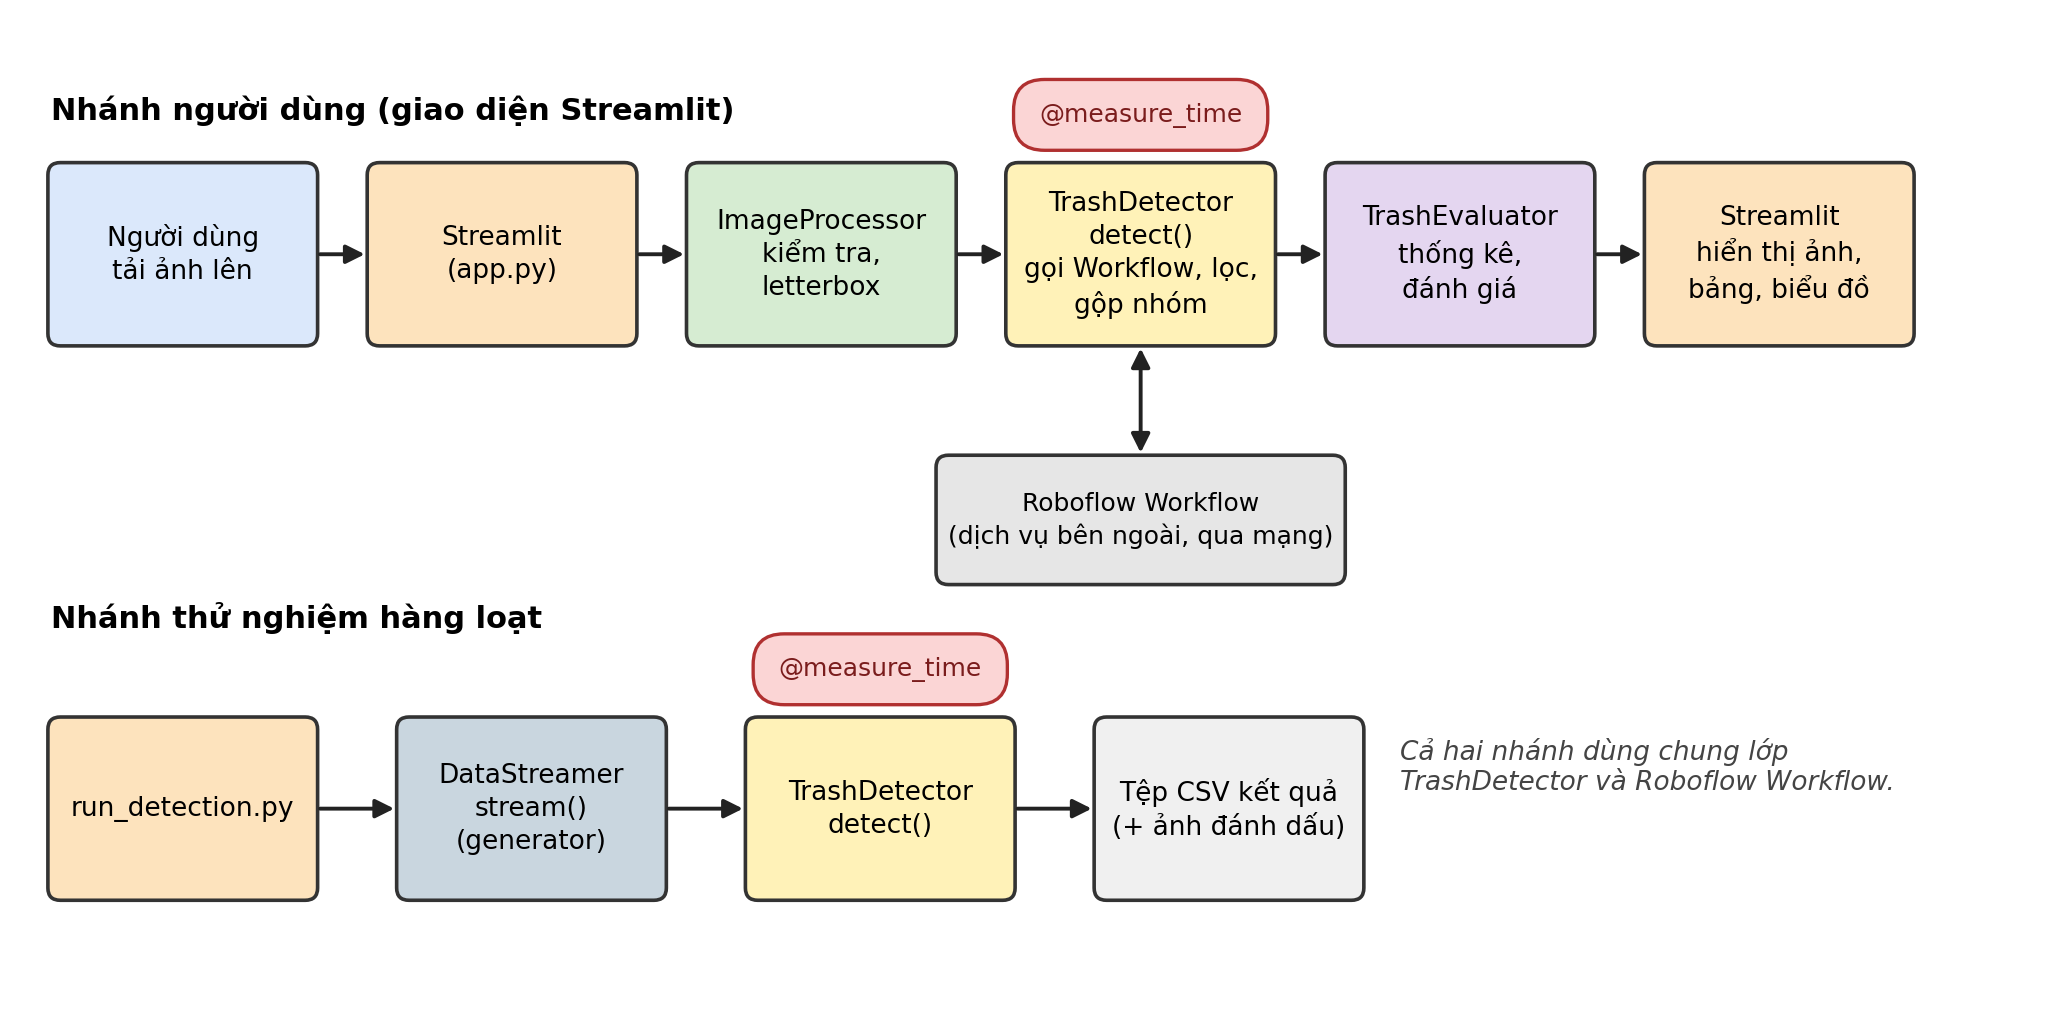
\includegraphics[width=1.0\textwidth]{so_do_luong.png} 
    \caption{Sơ đồ luồng xử lý}
    
\end{figure}

\subsection{Thiết kế các module chức năng theo kiến trúc OOP}
\subsubsection{ Module ImageProcessor}

ImageProcessor chịu trách nhiệm kiểm tra và chuẩn bị ảnh trước khi gửi đến mô hình. Lớp được khởi tạo với tham số target\_size (mặc định 640 điểm ảnh) và báo lỗi nếu giá trị này không lớn hơn 0.

Phương thức validate() kiểm tra ảnh đầu vào phải là mảng NumPy ba chiều (chiều cao, chiều rộng, số kênh màu) và mọi kích thước đều lớn hơn 0, nếu sai thì phát sinh ValueError với thông báo cụ thể. Phương thức process() thu phóng ảnh về vừa khung vuông target\_size × target\_size mà vẫn giữ nguyên tỉ lệ, đặt ảnh vào chính giữa và đệm phần còn lại bằng màu xám (giá trị 114). Cách làm này tránh làm méo vật thể so với việc kéo giãn ảnh.

Việc tách chức năng này thành một lớp riêng giúp quá trình chuẩn bị dữ liệu độc lập với quá trình nhận diện, dễ kiểm thử và dễ thay đổi.

\subsubsection{ Module TrashDetector}

TrashDetector là module kết nối với dịch vụ nhận diện. Khi khởi tạo, lớp nhận các tham số gồm ngưỡng tin cậy (mặc định 0.3), kích thước ảnh (640), ngưỡng IoU để loại khung trùng (0.6) và khóa API. Khóa API được đọc từ biến môi trường ROBOFLOW\_API\_KEY thay vì ghi trực tiếp trong mã nguồn, và hệ thống báo lỗi nếu chưa được thiết lập. Kết nối được tạo bằng InferenceHTTPClient của thư viện inference-sdk.

Phương thức detect() thực hiện các công việc sau:
\begin{enumerate}
    \item Chuyển ảnh đầu vào (đường dẫn, ảnh PIL hoặc mảng NumPy) về dạng mảng RGB.
    \item Gọi ImageProcessor để đưa ảnh về kích thước chuẩn, đồng thời tính hệ số thu phóng và phần lề đã đệm.
    \item Lưu ảnh thành tệp JPEG tạm thời, gửi đến Workflow cùng danh sách tên vật thể, sau đó xóa tệp tạm.
    \item Duyệt kết quả trả về, giữ các đối tượng có điểm tin cậy không thấp hơn ngưỡng và loại các kết quả trùng hệt nhau.
    \item Quy đổi tọa độ từ dạng tâm và kích thước (x, y, rộng, cao) trên ảnh đã gửi về dạng hai góc trên ảnh gốc, có trừ lề đệm và chia cho hệ số thu phóng.
    \item Gộp vật thể về bốn nhóm nhờ từ điển VAT\_THE, ví dụ plastic bottle thuộc nhóm Nhựa, glass bottle thuộc nhóm Thủy tinh, aluminum can thuộc nhóm Kim loại, cardboard và paper thuộc nhóm Giấy. Tên lạ được phân nhóm theo từ khóa, nếu không khớp thì xếp vào nhóm “Khác”.
    \item Loại các khung chồng lấn lên cùng một vật bằng chỉ số IoU, giữ lại khung có điểm tin cậy cao hơn.
\end{enumerate}

Mỗi đối tượng trả về gồm nhóm, tên vật thể bằng tiếng Việt, điểm tin cậy và tọa độ khung bao. Ngoài ra, phương thức ve\_ket\_qua() vẽ khung và nhãn tiếng Việt lên bản sao của ảnh, mỗi nhóm một màu riêng, có cơ chế tự bỏ dấu nếu máy không có phông chữ hỗ trợ tiếng Việt.

Việc tập trung toàn bộ thao tác gọi dịch vụ vào một lớp giúp các module khác không cần biết chi tiết cách kết nối. Khi cần đổi mô hình hay dịch vụ nhận diện, chỉ cần chỉnh sửa trong lớp này.

\subsubsection{ Module TrashEvaluator}

TrashEvaluator phân tích và tổng hợp kết quả do TrashDetector cung cấp. Module này không tham gia nhận diện mà chỉ xử lý thông tin đã có.

Phương thức evaluate() nhận danh sách đối tượng và trả về một bản đánh giá gồm: tổng số đối tượng; số lượng, tỉ lệ, độ tin cậy trung bình và độ tin cậy thấp nhất theo từng nhóm; nhóm xuất hiện nhiều nhất; độ tin cậy trung bình chung và mức tin cậy tương ứng; số đối tượng có độ tin cậy thấp cần kiểm tra lại; cùng các nhận xét bằng văn bản và gợi ý xử lý cho từng nhóm rác.

Mức tin cậy được phân thành ba bậc dựa trên hai ngưỡng có thể cấu hình: “Cao” khi điểm từ 0,70 trở lên, “Trung bình” khi từ 0,50 đến dưới 0,70 và “Thấp” khi dưới 0,50. Khi không phát hiện được vật thể nào, module trả về thông báo gợi ý dùng ảnh rõ hơn hoặc giảm ngưỡng tin cậy. Ngoài ra, phương thức so\_voi\_nhan\_chuan() cho phép so kết quả với nhãn đúng do người dùng cung cấp, phục vụ việc đo độ chính xác.

Cần lưu ý rằng điểm tin cậy do mô hình đưa ra không đồng nghĩa với xác suất chính xác tuyệt đối. Các mức “Cao”, “Trung bình”, “Thấp” chỉ mang tính tham khảo để hỗ trợ người dùng xem xét kết quả. Các gợi ý xử lý rác chỉ mang tính chung chung vì quy định phân loại rác khác nhau theo từng địa phương.

\subsubsection{ Module DataStreamer}

DataStreamer hỗ trợ thử nghiệm trên nhiều ảnh. Phương thức stream() là một generator, duyệt thư mục dữ liệu, lọc các tệp có phần mở rộng ảnh được hỗ trợ (JPG, JPEG, PNG, BMP, WebP), sắp xếp theo tên và lần lượt trả về đường dẫn từng ảnh bằng từ khóa yield. Module báo lỗi rõ ràng khi thư mục không tồn tại, đường dẫn không phải thư mục hoặc thư mục không có ảnh hợp lệ.

Cách tổ chức này giúp quy trình duyệt ảnh gọn gàng và không phải tạo sẵn kết quả xử lý của toàn bộ ảnh trong bộ nhớ. DataStreamer chỉ phục vụ thử nghiệm hàng loạt, không tham gia vào quá trình người dùng tải một ảnh trên giao diện.

\subsection{ Tích hợp các kỹ thuật Python nâng cao vào mã nguồn }

\subsubsection{ Lập trình hướng đối tượng (OOP)}

Hệ thống tổ chức các chức năng thành bốn lớp có nhiệm vụ rõ ràng: ImageProcessor quản lý việc kiểm tra và chuẩn bị ảnh, TrashDetector quản lý quá trình nhận diện, TrashEvaluator đảm nhận phân tích và đánh giá, DataStreamer phụ trách duyệt dữ liệu thử nghiệm. Mỗi lớp đóng gói dữ liệu cấu hình (như kích thước ảnh, ngưỡng tin cậy) cùng các phương thức xử lý liên quan. Nhờ vậy, các thành phần tập trung vào nhiệm vụ của mình, giảm sự phụ thuộc lẫn nhau và dễ thay thế hoặc mở rộng.

\subsubsection{ Decorator đo thời gian xử lý}

Decorator measure\_time bổ sung chức năng đo thời gian thực thi cho một hàm mà không cần sửa logic bên trong hàm đó. Decorator ghi lại thời điểm trước và sau khi gọi hàm, tính hiệu hai giá trị và in ra thời gian xử lý. Nhờ functools.wraps, hàm sau khi được bọc vẫn giữ nguyên tên và mô tả ban đầu; nhờ khối finally, thời gian vẫn được ghi nhận kể cả khi hàm phát sinh ngoại lệ.

Decorator được áp dụng cho phương thức detect() của TrashDetector như sau:

\begin{lstlisting}[language=Python, numbers=none, caption={Áp dụng Decorator measure\_time cho phương thức detect()}]
class TrashDetector:
    # ...
    @measure_time
    def detect(self, image, confidence_threshold=None):
        ...
\end{lstlisting}

Cần lưu ý rằng thời gian đo được bao gồm cả độ trễ đường truyền khi gọi dịch vụ nhận diện, nên không phản ánh riêng tốc độ suy luận của mô hình.
\subsubsection{Generator trong quá trình nạp dữ liệu}

Generator được dùng để duyệt lần lượt các ảnh trong thư mục thử nghiệm. Thay vì trả về toàn bộ danh sách cùng lúc, hàm cung cấp từng đường dẫn khi chương trình yêu cầu.

\begin{lstlisting}[language=Python, numbers=none, caption={Generator trong DataStreamer}]
def stream(self) -> Iterator[Path]:
    """Lan luot yield duong dan tung anh, sap xep theo ten."""
    # ... kiem tra thu muc, loc va sap xep anh ...
    for path in image_paths:
        yield path
\end{lstlisting}

Cách này giúp quá trình duyệt dữ liệu dễ tổ chức và phù hợp với quy trình kiểm thử nhiều ảnh.

\subsubsection{ Docstring và Type Hints}

Docstring mô tả mục đích, tham số và giá trị trả về của lớp và hàm, giúp các thành viên hiểu mã nguồn của nhau. Type Hints khai báo kiểu dữ liệu dự kiến của tham số và giá trị trả về, giúp mã dễ đọc hơn và hỗ trợ công cụ kiểm tra kiểu.

\begin{lstlisting}[language=Python, numbers=none, caption={Docstring và Type Hints trong ImageProcessor}]
def process(self, image: np.ndarray) -> np.ndarray:
    """Dua anh ve khung vuong target_size x target_size (letterbox).

    Args:
        image: Anh dang mang NumPy (cao, rong, kenh mau).
    Returns:
        Anh da thu phong va giua ti le va dem mau xam 
    """
\end{lstlisting}


Tuy nhiên, Type Hints chỉ có tác dụng khai báo và hỗ trợ công cụ kiểm tra, không tự động bảo đảm dữ liệu lúc chạy luôn đúng kiểu. Vì vậy, ImageProcessor vẫn kiểm tra dữ liệu thực tế trong validate().

\subsection{Xây dựng giao diện tương tác người dùng bằng Streamlit}

\subsubsection{Mục tiêu thiết kế giao diện}
Giao diện được xây dựng bằng Streamlit trong tệp \texttt{app.py}, giúp người dùng thao tác với hệ thống ngay trên trình duyệt mà không cần gọi trực tiếp các hàm Python. Giao diện hướng đến sự đơn giản, tập trung vào ba thao tác chính: tải ảnh lên, thực hiện nhận diện và xem kết quả. Bên cạnh đó, giao diện cho phép người dùng điều chỉnh hai tham số ảnh hưởng đến kết quả là ngưỡng độ tin cậy và kích thước ảnh, đồng thời xuất kết quả ra tệp để sử dụng lại.

\subsubsection{Các thành phần giao diện}
Giao diện ứng dụng gồm các thành phần sau:
\begin{enumerate}
    \item Thanh bên: gồm thanh trượt chọn ngưỡng độ tin cậy (từ 0,05 đến 0,95, bước 0,05, mặc định 0,30), thanh chọn kích thước ảnh (320, 416, 512, 640, 800, 960 hoặc 1024 điểm ảnh, mặc định 640) và thông báo trạng thái kết nối dịch vụ nhận diện. Nếu chưa có khóa API, thanh bên hiển thị thông báo lỗi kèm hướng dẫn thiết lập.
    \item Khu vực tải ảnh: cho phép chọn một tệp ảnh định dạng PNG, JPG, JPEG hoặc WebP. Bên cạnh là phần hiển thị bốn nhóm rác mà hệ thống hỗ trợ (Thủy tinh, Kim loại, Giấy, Nhựa).
    \item Xem trước ảnh và nút ``Phân tích ảnh'': sau khi tải lên, ảnh được hiển thị để người dùng kiểm tra trước khi thực hiện nhận diện.
    \item Các chỉ số tổng hợp: số vật thể phát hiện, số nhóm phát hiện, độ tin cậy trung bình và thời gian xử lý.
    \item Khu vực kết quả: ảnh gốc đặt cạnh ảnh đã đánh dấu khung và nhãn tiếng Việt để người dùng dễ so sánh.
    \item Thống kê theo nhóm: biểu đồ cột số lượng vật thể theo nhóm và bảng chi tiết gồm nhóm, vật thể, độ tin cậy và tọa độ khung bao.
    \item Đánh giá kết quả: do \texttt{TrashEvaluator} cung cấp, gồm nhóm chính, mức tin cậy chung, số vật cần kiểm tra lại, các nhận xét bằng văn bản, bảng thống kê theo nhóm (số lượng, tỉ lệ, độ tin cậy trung bình và thấp nhất) và gợi ý xử lý cho từng nhóm rác ở dạng có thể mở rộng. Các gợi ý này chỉ mang tính tham khảo.
    \item Xuất dữ liệu: nút tải kết quả nhận diện dạng CSV (mã hóa UTF-8 để mở bằng Excel không lỗi tiếng Việt) và nút tải ảnh đã đánh dấu dạng PNG.
    \item Thông báo trạng thái: cảnh báo khi chưa có khóa API, khi ảnh không đọc được, khi không phát hiện được vật thể nào hoặc khi việc nhận diện gặp lỗi.
\end{enumerate}

\begin{figure}[H]
    \centering
    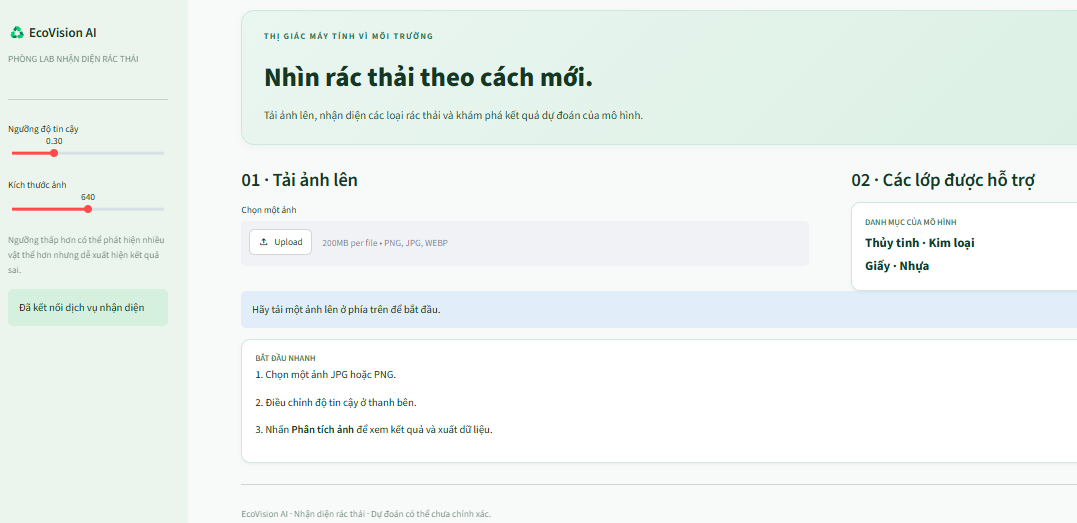
\includegraphics[width=0.95\textwidth]{giao diện.png}
    \caption{Giao diện ứng dụng nhận diện rác thải}
\end{figure}

\subsubsection{Quy trình hoạt động của giao diện}
Khi người dùng tải ảnh lên, Streamlit đọc ảnh, chuyển sang hệ màu RGB và hiển thị bản xem trước. Nếu ảnh không đọc được, giao diện báo lỗi và dừng xử lý. Khi người dùng nhấn nút ``Phân tích ảnh'', giao diện kiểm tra khóa API rồi khởi tạo \texttt{TrashDetector} với ngưỡng tin cậy và kích thước ảnh đã chọn. Đối tượng \texttt{TrashDetector} được lưu bộ nhớ đệm bằng \texttt{st.cache\_resource} theo cặp tham số này, nên không phải khởi tạo lại ở mỗi lần bấm nút khi tham số không đổi.

Tiếp theo, giao diện gọi phương thức \texttt{detect()} để nhận diện, gọi \texttt{ve\_ket\_qua()} để vẽ khung và nhãn lên ảnh, rồi chuyển danh sách đối tượng cho \texttt{TrashEvaluator.evaluate()} để lấy kết quả đánh giá. Cuối cùng, giao diện hiển thị các chỉ số, ảnh kết quả, bảng thống kê và các nút xuất dữ liệu. Thời gian xử lý hiển thị trên giao diện được tính từ lúc bắt đầu nhận diện đến khi hoàn tất phần đánh giá, nên bao gồm cả bước vẽ khung và đánh giá, và có thể lớn hơn một chút so với thời gian của riêng phương thức \texttt{detect()} ghi trong tệp CSV khi chạy hàng loạt.

Khi không phát hiện được vật thể nào, ứng dụng hiển thị thông báo gợi ý giảm nhẹ ngưỡng tin cậy thay vì tự gán ảnh vào một nhóm. Khi việc gọi dịch vụ gặp lỗi, giao diện hiển thị thông báo lỗi và chi tiết ngoại lệ để thuận tiện cho việc kiểm tra. Khóa API được đọc từ biến môi trường \texttt{ROBOFLOW\_API\_KEY} hoặc từ tệp \texttt{.streamlit/secrets.toml} chứ không được ghi trực tiếp trong mã nguồn. Việc tách giao diện khỏi các module xử lý giúp có thể thay đổi giao diện mà không phải viết lại phần nhận diện.

\subsection{Tổng kết chương}
Chương 3 đã trình bày kiến trúc tổng thể, luồng xử lý dữ liệu và thiết kế các module của hệ thống nhận diện rác. Hệ thống gồm bốn lớp \texttt{ImageProcessor}, \texttt{TrashDetector}, \texttt{TrashEvaluator} và \texttt{DataStreamer}, mỗi lớp đảm nhận một nhiệm vụ riêng: chuẩn bị ảnh, gọi dịch vụ nhận diện và xử lý kết quả, đánh giá kết quả, và nạp ảnh cho thử nghiệm hàng loạt. Bước phát hiện đối tượng do Roboflow Workflow thực hiện, còn các thành phần Python của nhóm kết nối, xử lý và trình bày kết quả.

Bên cạnh đó, chương mô tả cách các kỹ thuật Python nâng cao được áp dụng vào mã nguồn: OOP để tổ chức các lớp, Decorator \texttt{measure\_time} để đo thời gian thực thi phương thức \texttt{detect()}, Generator trong \texttt{DataStreamer} để duyệt ảnh lần lượt, cùng Docstring và Type Hints để mô tả mã nguồn. Giao diện Streamlit cho phép người dùng tải ảnh, điều chỉnh tham số, xem kết quả cùng phần đánh giá và xuất dữ liệu.

Cấu trúc chia module rõ ràng là nền tảng cho phần thực nghiệm. Chương 4 sẽ trình bày kết quả chạy hệ thống trên tập ảnh thử nghiệm, kèm thời gian xử lý và phân tích các trường hợp nhận diện tốt và chưa tốt.

\section{ KẾT QUẢ THỰ NGHIỆM VÀ ĐÁNH GIÁ}

\subsection{ Chuẩn bị tập dữ liệu thử nghiệm}
\begin{itemize}
    \item Nguồn ảnh và tiêu chí lựa chọn ảnh.
    \item Phân bố ảnh theo nhóm: nhựa, giấy, kim loại, thủy tinh, nhiều loại lẫn nhau.
    \item Phương pháp xác định nhãn đúng.
    \item Hình ảnh mẫu trong tập dữ liệu.
    \item Điều kiện thực nghiệm: ngưỡng tin cậy, kích thước ảnh, cấu hình máy, ngày chạy và kết nối Internet.
\end{itemize}

\subsection { Kết quả nhận diện và thời gian xử lý}
\begin{itemize}
    \item Quy trình chạy thử nghiệm bằng \texttt{DataStreamer} và \texttt{TrashDetector}.
    \item Đo thời gian xử lý bằng decorator \texttt{@measure\_time}.
    \item Kết quả nhận diện từng ảnh từ \texttt{detection\_summary.csv}.
    \item Các chỉ số tổng hợp:
    \begin{itemize}
        \item Số ảnh nhận diện đúng.
        \item Số ảnh đáp ứng tiêu chí nhận diện đúng nghiêm ngặt.
        \item Số ảnh không phát hiện được vật thể.
        \item Thời gian xử lý trung bình, nhỏ nhất và lớn nhất.
        \item Độ tin cậy trung bình theo từng nhóm.
    \end{itemize}
    \item Biểu đồ thống kê kết quả nhận diện.
    \item So sánh ảnh gốc với ảnh sau nhận diện.
    \item Kết quả hiển thị trên giao diện Streamlit và phần đánh giá của \texttt{TrashEvaluator}.
    \item Nhận xét về thời gian xử lý, bao gồm độ trễ mạng.
\end{itemize}

\subsection { Phân tích kết quả thực nghiệm}
\begin{itemize}
    \item Các trường hợp nhận diện tốt.
    \item Các trường hợp nhận diện chưa tốt:
    \begin{itemize}
        \item Không phát hiện được vật thể.
        \item Phát hiện trùng hoặc quá nhiều vật thể.
        \item Nhầm nhóm rác trong ảnh có nhiều loại.
    \end{itemize}
    \item Ảnh hưởng của ngưỡng tin cậy $0.2$, $0.3$, $0.5$.
    \item Ảnh hưởng của kích thước ảnh 640 và 960.
    \item Đánh giá vai trò của \texttt{TrashEvaluator}.
    \item Hạn chế của kết quả và phạm vi áp dụng.
\end{itemize}

\subsection {Tổng kết chương}
\begin{itemize}
    \item Tóm tắt kết quả thực nghiệm.
    \item Nêu những ưu điểm và hạn chế chính của hệ thống.
\end{itemize}

\section{KẾT LUẬN VÀ HƯỚNG PHÁT TRIỂN}

\subsection{ Kết quả đạt được của đề tài}
\begin{itemize}
    \item Đối chiếu bảy mục tiêu tại Mục 1.2.2.
    \item Các chức năng đã xây dựng:
    \begin{itemize}
        \item Nhận diện bốn nhóm rác.
        \item Vẽ khung bao và nhãn tiếng Việt.
        \item Thống kê và đánh giá độ tin cậy.
        \item Xuất kết quả CSV và ảnh.
        \item Xử lý hàng loạt bằng \texttt{run\_detection.py}.
    \end{itemize}
    \item Các kỹ thuật Python nâng cao:
    \begin{itemize}
        \item OOP: \texttt{ImageProcessor}, \texttt{TrashDetector}, \texttt{TrashEvaluator}, \texttt{DataStreamer}.
        \item Decorator: \texttt{measure\_time}.
        \item Generator: \texttt{DataStreamer.stream()}.
        \item Docstring và Type Hints.
    \end{itemize}
    \item Bài học kinh nghiệm.
    \item Các số liệu thực nghiệm tiêu biểu từ Chương 4.
\end{itemize}

\subsection {Các mặt hạn chế}
\begin{itemize}
    \item Hạn chế về tập dữ liệu.
    \item Hạn chế về khả năng nhận diện của Roboflow Workflow.
    \item Phụ thuộc Internet và khóa API.
    \item Thời gian xử lý và độ trễ mạng.
    \item Chưa đánh giá đầy đủ tình trạng rác như sạch, bẩn, vỡ, ẩm.
    \item Chưa có kiểm thử tự động đầy đủ.
\end{itemize}

\subsection{ Hướng nghiên cứu và phát triển tiếp theo}
\begin{itemize}
    \item Xây dựng tập dữ liệu riêng và nghiên cứu mô hình nhận diện chạy ngoại tuyến.
    \item Phát triển nhận diện video thời gian thực qua webcam.
    \item Mở rộng nhóm rác và phân loại
    \item Bổ sung hướng dẫn phân loại rác theo quy định địa phương.
    \item Viết unit test và đóng gói ứng dụng để triển khai.
\end{itemize}

\subsection{ Tổng kết chương}
\begin{itemize}
    \item Khái quát kết quả đề tài.
    \item Nêu định hướng hoàn thiện và phát triển hệ thống trong tương lai.
\end{itemize}

\newpage

\begin{center}
    {\fontsize{16}{20}\selectfont \textbf{TÀI LIỆU THAM KHẢO}}\\[0.5cm]
\end{center}

\noindent [1] NumPy Developers, \textit{NumPy Documentation}.
Available at: \url{https://numpy.org/doc/stable/}.

\noindent [2] Pillow Contributors, \textit{Pillow Documentation}.
Available at: \url{https://pillow.readthedocs.io/}.

\noindent [3] Python Software Foundation,
\textit{PEP 8 -- Style Guide for Python Code}.
Available at: \url{https://peps.python.org/pep-0008/}.

\noindent [4] Python Software Foundation,
\textit{Python 3 Documentation}.
Available at: \url{https://docs.python.org/3/}.

\noindent [5] Roboflow, \textit{Roboflow Documentation}.
Available at: \url{https://docs.roboflow.com/}.

\noindent [6] Roboflow, \textit{Roboflow Inference Documentation}.
Available at: \url{https://inference.roboflow.com/}.

\noindent [7] Streamlit, \textit{Streamlit Documentation}.
Available at: \url{https://docs.streamlit.io/}.
\end{document}